\section{Análisis}

\subsection{Características estructurales}
\label{subsec:structure}

Observando de nuevo la red de la Figura \ref{fig:filtered}, podemos distinguir
tres agrupaciones de nodos de usuarios. La más grande y, a su vez, más
reconocible, es la que se encuentra en el centro de la Figura, estando las otras
dos agrupaciones a su derecha y menos claras debido a su tamaño.

En estas grupaciones, siempre encontramos en el centro una pareja de nodos que
se corresponden con un \textit{tweet} y su autor, siendo los nodos agrupados a
su alrededor los usuarios que han interaccionado con él. A primera vista,
podríamos decir que estos tres \textit{tweets} que están en los centros de estas
agrupaciones son los más relevantes, y sus autores los usuarios más influyentes,
pero vamos a esperar a analizar distintas métricas de la red para poder realizar
una aserción más fundada.

Por último, decir que tenemos también pequeñas componentes aisladas de 3 o 4
nodos. Se trata de \textit{tweets} sueltos con los que han interaccionado 1 o 2
usuarios. Esta fragmentación es muy común en redes como ésta.

\subsection{Métricas globales}

Usando \textit{Gephi}, se calculan directamente algunas medidas globales de la
red, las cuáles se pueden encontrar en el cuadro \ref{tab:metrics}.

\begin{table}[h!]
    \caption{Medidas obtenidas de la red}
    \label{tab:metrics}
    \begin{center}
        \begin{tabular}{ |p{8cm}|c| }
            \hline
            \textbf{Medida}                                              & \textbf{Valor} \\
            \hline
            Número de nodos $N$                                          & 2970           \\
            \hline
            Número de enlaces $L$                                        & 6705           \\
            \hline
            Densidad del grafo $L/L_{max}$                               & 0.001          \\
            \hline
            Grado medio $\langle k \rangle$                              & 2.258          \\
            \hline
            Diámetro $d_{max}$                                           & 14             \\
            \hline
            Distancia media $\langle d \rangle$                          & 5.2425         \\
            \hline
            Distancia media para la red aleatoria equivalente $\langle
            d_{aleatoria} \rangle$                                       & 9.8177         \\
            \hline
            Coeficiente medio de \textit{clustering} $\langle C \rangle$ & 0.380          \\
            \hline
            Coeficiente medio de \textit{clustering} para la red aleatoria
            equivalente $\langle C_{aleatoria} \rangle$                  & 0.00076        \\
            \hline
            Número de componentes conexas                                & 28             \\
            \hline
            Número de nodos de la componente gigante (y \%)              & 2868 (96.57\%) \\
            \hline
            Número de enlaces de la componente gigante (y \%)            & 6586 (98.23\%) \\
            \hline
        \end{tabular}
    \end{center}
\end{table}

\subsection{Propiedades}

A partir de las distintas métricas de la red, vamos a caracterizar la misma para
comprobar si se cumplen algunas propiedades conocidas. Para empezar, vamos a
observar las distribuciones de grados para comprobar si la red es libre de
escala. Al tratarse de una red dirigida, debemos considerar tanto el grado de
entrada como el de salida. Las distribuciones de estos grados las encontramos en
las gráficas de las Figuras \ref{fig:indegree-distribution-plot} y
\ref{fig:outdegree-distribution-plot}, respectivamente.

\begin{figure}
    \centering
    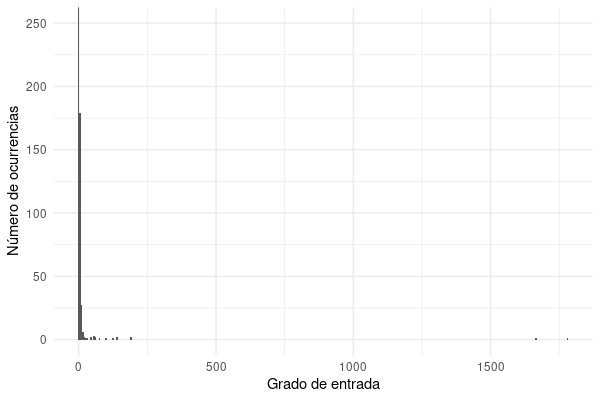
\includegraphics[width=\textwidth]{images/plots/indegree.png}
    \caption{Distribución del grado de entrada}
    \label{fig:indegree-distribution-plot}
\end{figure}

\begin{figure}
    \centering
    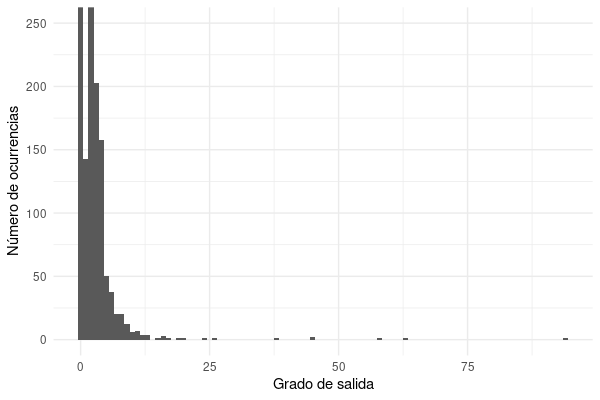
\includegraphics[width=\textwidth]{images/plots/outdegree.png}
    \caption{Distribución del grado de salida}
    \label{fig:outdegree-distribution-plot}
\end{figure}

Observando ambas gráficas, vemos como las distribuciones siguen la ley de la
potencia, por lo que podemos afirmar que la red que estamos estudiando es libre
de escala. En este tipo de redes, tenemos unos pocos nodos con un gran número de
enlaces (\textit{hubs}), muy por encima del grado medio de la red.

También es común en redes sociales que sean redes de mundo pequeño. En estas
redes, aunque la mayoría de nodos no son vecinos entre sí, se puede llegar a
cualquier nodo desde otro en un número relativamente bajo de saltos. Para que
una red sea de mundo pequeño, su distancia media debe tener una escala
logarítmica respecto al tamaño de la red, tal y como se indica en la ecuación
(\ref{eq:small-worlds}).

\begin{equation}
    \langle d \rangle = \frac{\ln(N)}{\ln(\langle k \rangle)}
    \label{eq:small-worlds}
\end{equation}

El resultado de este cálculo para nuestra red es 9.8177, un valor superior a la
distancia media de la red, que es de 5.2425. Al estar por debajo de esta escala,
podríamos decir ya que se trata de una red de mundo pequeño. No obstante, vamos
a comprobar también la escala que define las redes de mundo ultra-pequeño para
confirmarlo.

Aplicamos entonces la ecuación (\ref{eq:ultra-small-worlds}), que es la que
define la distancia media en una red de este tipo, obteniendo un valor de
3.8462. Este valor es inferior a la distancia media de nuestra red, por lo que
no se trata de una red de mundo ultra-pequeño, si no que es de mundo pequeño.

\begin{equation}
    \langle d \rangle = \frac{\ln(N)}{\ln(\ln(N))}
    \label{eq:ultra-small-worlds}
\end{equation}

Por último, vamos a estudiar la transitividad de la red. En redes sociales como
la nuestra, la transitividad lleva a grafos más densos, es decir, más cercanos a
un grafo completo. Por tanto, podemos medir esta transitividad fijándonos en
como de cerca está el grafo de ser completo. Para ello, usamos el coeficiente de
\textit{clustering} de los nodos, que mide la transitividad de la red a nivel de
nodo. En la Figura \ref{fig:clustering-plot} encontramos una gráfica de la
distribución de este coeficiente.

\begin{figure}
    \centering
    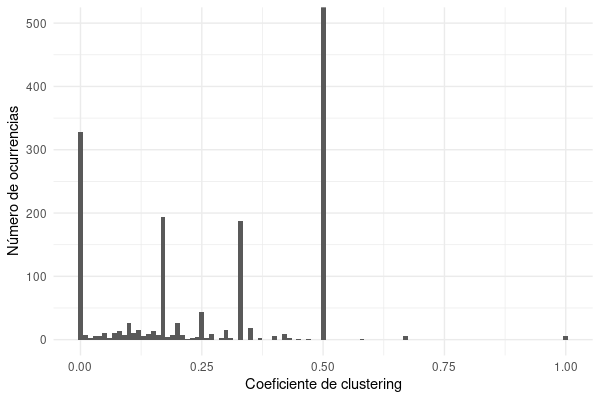
\includegraphics[width=\textwidth]{images/plots/clustering.png}
    \caption{Distribución del coeficiente de \textit{clustering}}
    \label{fig:clustering-plot}
\end{figure}

Normalmente, en redes sociales consideraríamos alto un valor medio del
coeficiente de \textit{clustering} de en torno a 0.6, lo que indicaría tiene una
transitividad alta. En la red que se está estudiando, este valor medio es de
0.38, con lo que no es especialmente transitiva, pero tampoco consideramos que
sea un valor demasiado bajo.

\subsection{Actores principales}
\label{subsec:actors}

Para obtener los actores principales de la red, vamos a comenzar observando
tanto el soporte (grado de entrada) como la influencia (grado de salida) de los
nodos. En la Figura \ref{fig:indegree-graph} vemos que los nodos con mayor
soporte son el \textit{tweet} con más interacciones y su autora,
\textbf{@elenarnz7}. Esta usuaria es la que más interacciones ha recibido y, por
tanto, es la actriz principal de la red según el soporte. Atendiendo a la
influencia, cuya representación sobre la red encontramos en la Figura
\ref{fig:outdegree-graph}, tenemos que \textbf{@garccabrerizo} es el actor más importante.

\begin{figure}
    \centering
    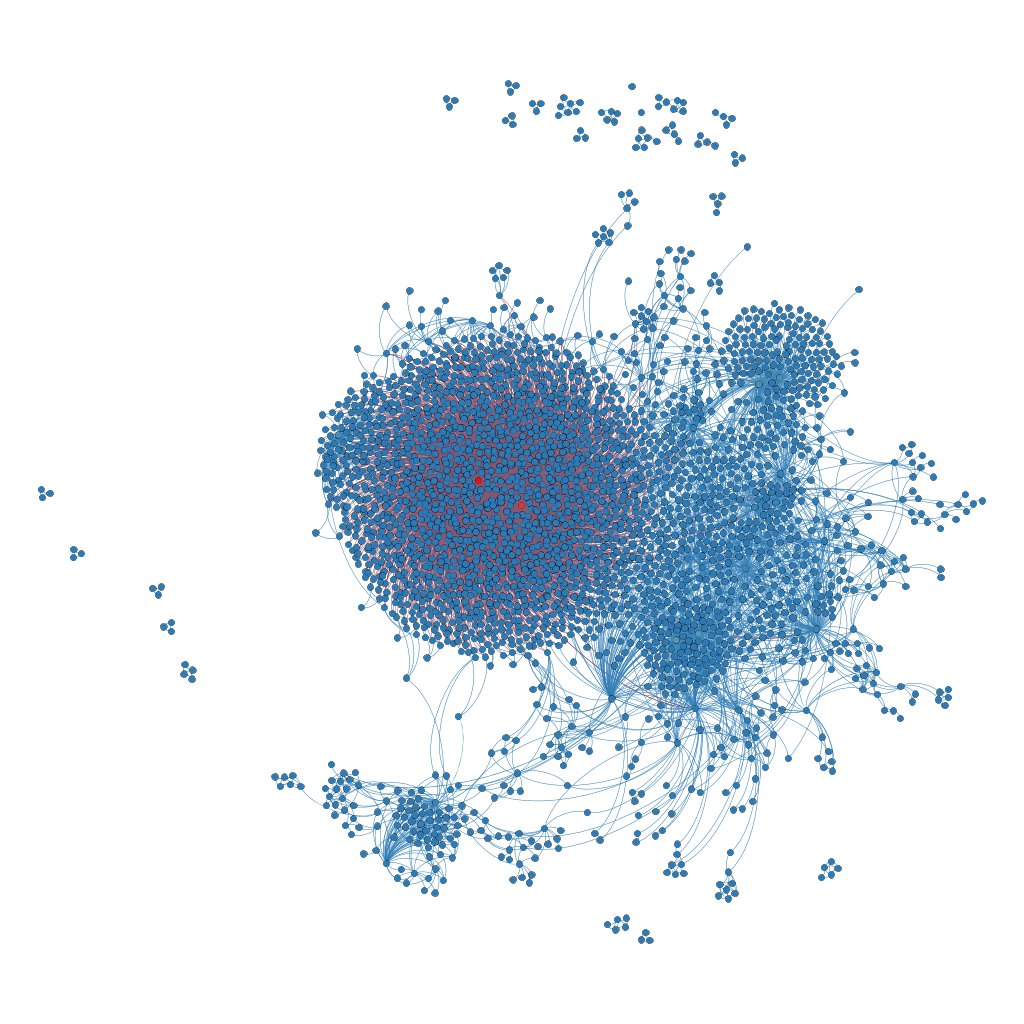
\includegraphics[width=\textwidth]{images/graph/indegree.png}
    \caption{Red coloreada según el soporte (rojo indica un mayor valor y azul, menor)}
    \label{fig:indegree-graph}
\end{figure}

\begin{figure}
    \centering
    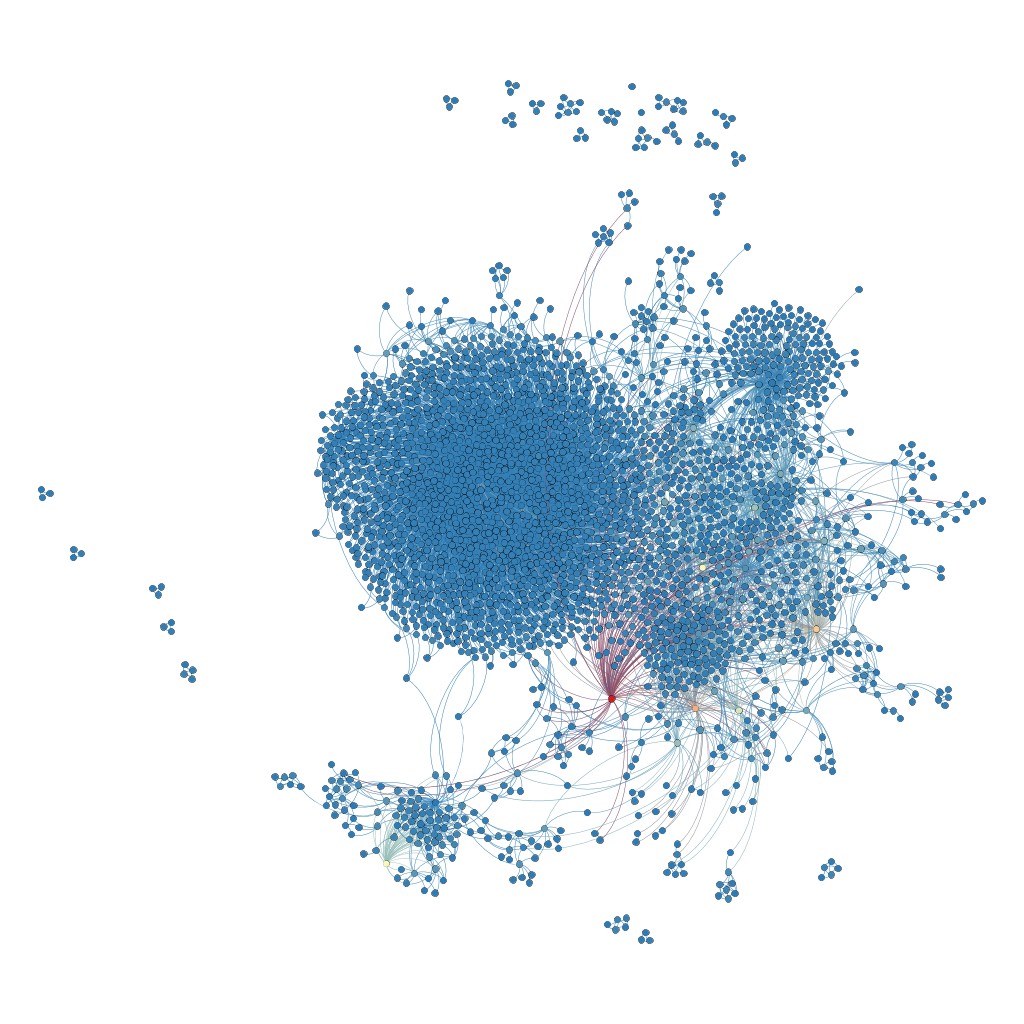
\includegraphics[width=\textwidth]{images/graph/outdegree.png}
    \caption{Red coloreada según la influencia (rojo indica un mayor valor y azul, menor)}
    \label{fig:outdegree-graph}
\end{figure}

El grado no captura las <<corredurías>>, por lo que nos tenemos que fijar en
otras medidas de centralidad de los nodos. La primera de estas medidas de
centralidad que vamos a observar es la de intermediación. Esta métrica indica,
para cada nodo, la proporción de caminos mínimos de la red que pasan por él.
Así, podemos identificar nodos que son críticos para la transmisión de la
información. En la Figura \ref{fig:betweenness-centrality-plot} encontramos la
distribución de esta medida de centralidad en la que, como vemos, la gran
mayoría de nodos tienen un valor muy bajo. Esto lo podemos corroborar observando
la red coloreada según estos valores en la Figura
\ref{fig:betweenness-centrality-graph}. Los nodos con mayor intermediación
corresponden a los usuarios \textbf{@ugrenfurecida}, \textbf{@elenavg99},
\textbf{@garccabrerizo} y \textbf{@saseamaro}. Debemos hacer mención especial a
la cuenta de la UGR, \textbf{@canalugr}, la cuál, aunque no es de los valores
más altos, sí que tiene un valor más alto que la mayoría y se puede ver en la
Figura \ref{fig:betweenness-centrality-graph} como uno de los nodos de color
amarillo pálido.

\begin{figure}
    \centering
    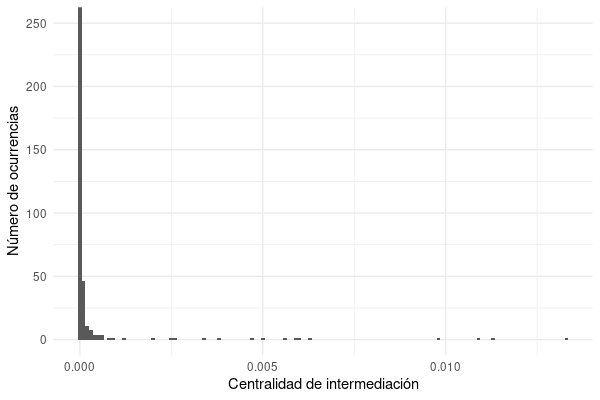
\includegraphics[width=\textwidth]{images/plots/betweenness-centrality.png}
    \caption{Distribución de la centralidad de intermediación}
    \label{fig:betweenness-centrality-plot}
\end{figure}

\begin{figure}
    \centering
    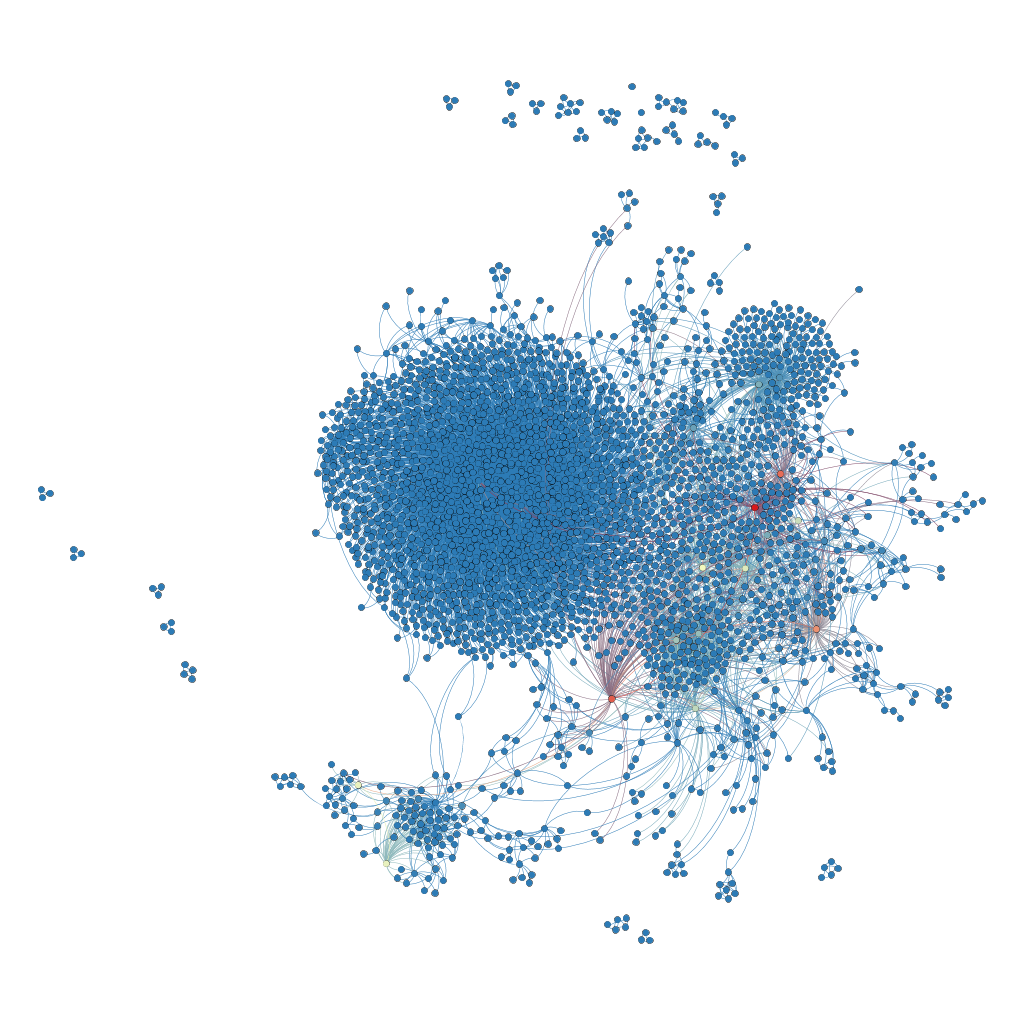
\includegraphics[width=\textwidth]{images/graph/betweenness-centrality.png}
    \caption{Red coloreada según la centralidad de intermediación (rojo indica un mayor valor y azul, menor)}
    \label{fig:betweenness-centrality-graph}
\end{figure}

Ahora, vamos a observar la centralidad de cercanía. Como su propio nombre
indica, esta métrica da especial importancia a que los nodos se encuentren cerca
del centro de la red, basándose en la distancia de un nodo a otros. En la Figura
\ref{fig:closeness-centrality-plot} tenemos la gráfica de distribución de esta
métrica y, en la \ref{fig:closeness-centrality-graph}, la red coloreada en base
a ella. Como era de esperar, los nodos con mayor valor de cercanía son los que
se encuentran en la agrupación de nodos principal, la relativa al \textit{tweet}
con más interacciones que hemos capturado. Estos son los actores más centrales.

\begin{figure}
    \centering
    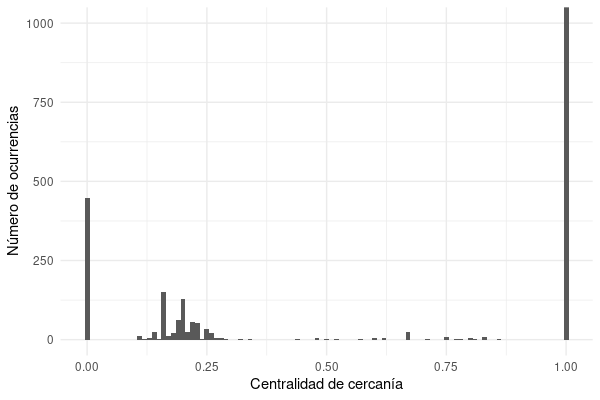
\includegraphics[width=\textwidth]{images/plots/closeness-centrality.png}
    \caption{Distribución de la centralidad de cercanía}
    \label{fig:closeness-centrality-plot}
\end{figure}

\begin{figure}
    \centering
    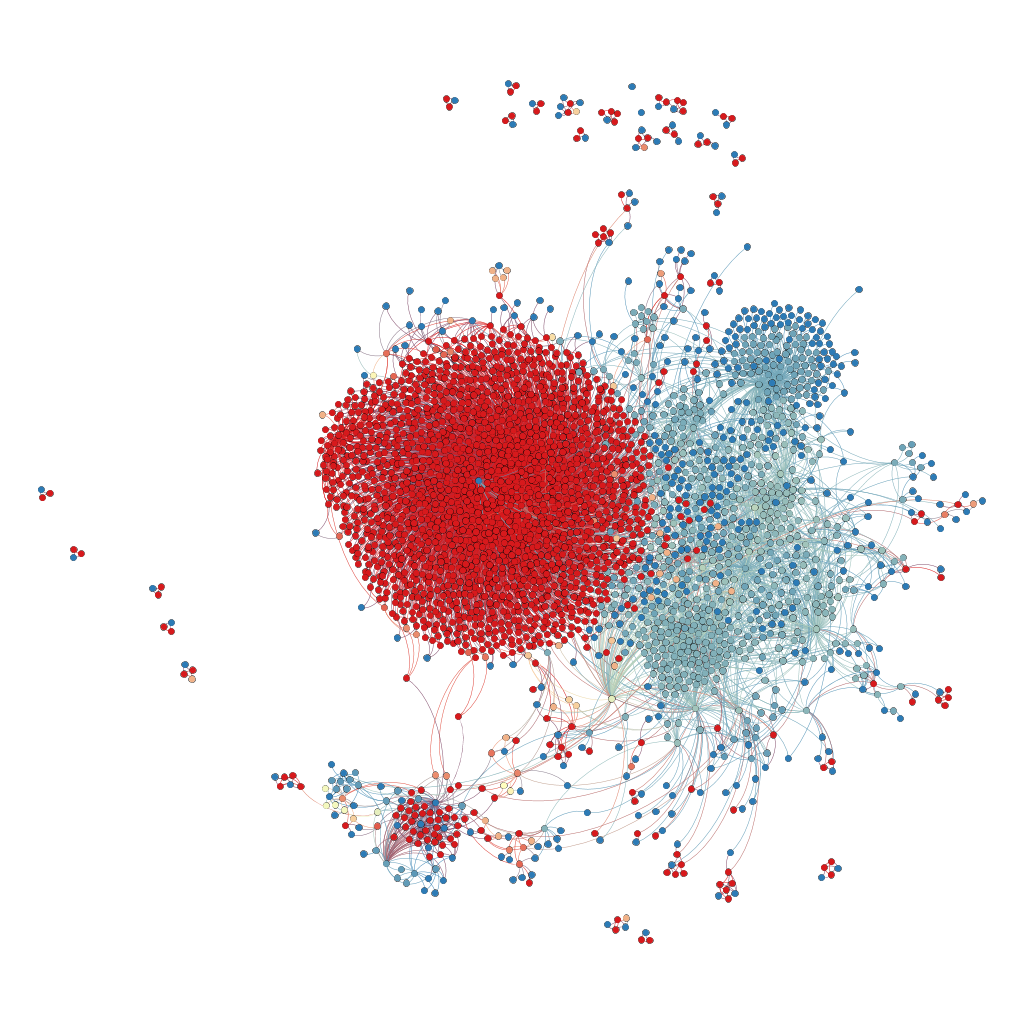
\includegraphics[width=\textwidth]{images/graph/closeness-centrality.png}
    \caption{Red coloreada según la centralidad de cercanía (rojo indica un mayor valor y azul, menor)}
    \label{fig:closeness-centrality-graph}
\end{figure}

Por el contrario, podemos identificar a los actores periféricos fijándonos en
los valores de excentricidad, que es la métrica inversa a la cercanía. La
distribución de esta métrica la encontramos reflejada en la Figura
\ref{fig:eccentricity-plot}. Fijándonos en la representación de la red coloreada
en base a esta métrica, que tenemos en la Figura \ref{fig:eccentricity-graph},
vemos como los principales actores periféricos son los usuarios que se agrupan
en torno a un conjunto de \textit{tweets} aislados al sur de la red, además de
los nodos relativos a los otros dos \textit{tweets} con más interacciones que se
han capturado. Algunos de estos nodos son los mismos usuarios que tenían un
mayor valor de intermediación.

\begin{figure}
    \centering
    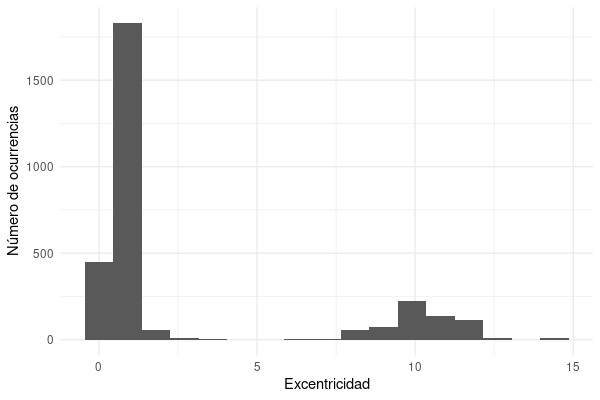
\includegraphics[width=\textwidth]{images/plots/eccentricity.png}
    \caption{Distribución de la excentricidad}
    \label{fig:eccentricity-plot}
\end{figure}

\begin{figure}
    \centering
    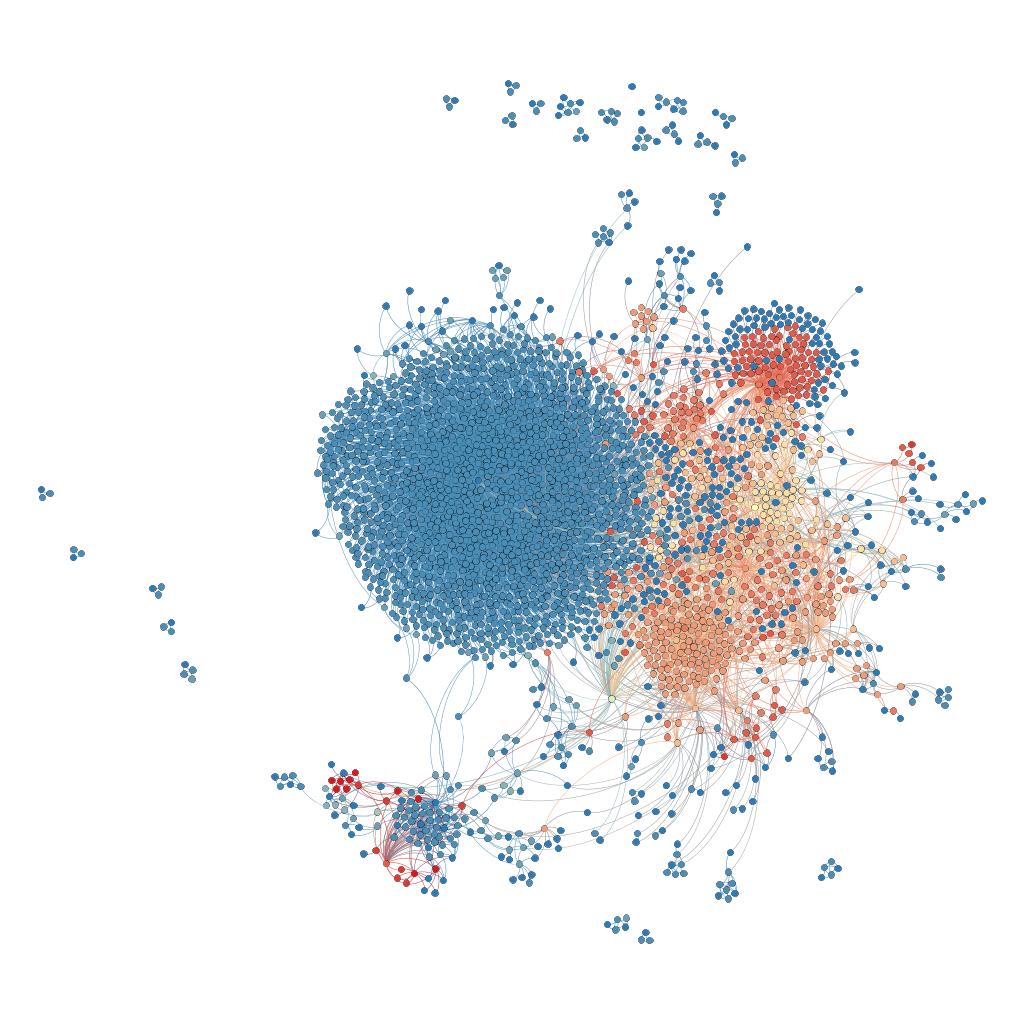
\includegraphics[width=\textwidth]{images/graph/eccentricity.png}
    \caption{Red coloreada según la excentricidad (rojo indica un mayor valor y azul, menor)}
    \label{fig:eccentricity-graph}
\end{figure}

Como última medida para la identificación de los actores principales, podemos
considerar la centralidad de vector propio. Esta medida se basa en la idea de
que la centralidad de un nodo concreto depende de cómo de centrales sean sus
vecinos. Por tanto, no es sorpresa que los nodos con mayor valor de esta métrica
sean el \textit{tweet} con más interacciones de la red y su autora,
\textbf{@elenarnz7}, ya que se encuentran conectados con todos los nodos que
tienen mayor valor de cercanía, tal y como veíamos en la Figura
\ref{fig:closeness-centrality-graph}. Una representación de la red coloreada
según la centralidad de vector propio se puede ver en la Figura
\ref{fig:eigenvector-centrality-graph}, la cuál es idéntica a la representación
coloreada según el grado de entrada.

\begin{figure}
    \centering
    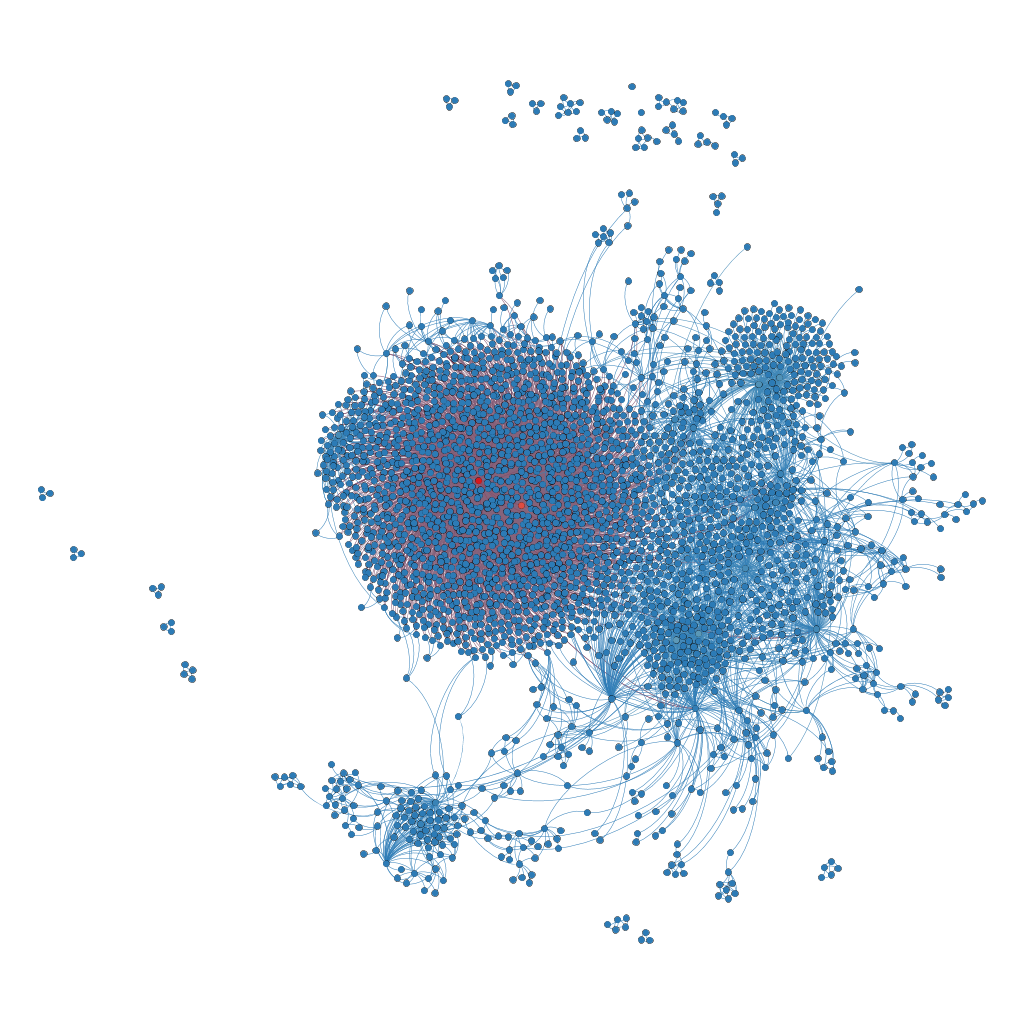
\includegraphics[width=\textwidth]{images/graph/eigenvector-centrality.png}
    \caption{Red coloreada según la centralidad de vector propio (rojo indica un mayor valor y azul, menor)}
    \label{fig:eigenvector-centrality-graph}
\end{figure}

\subsection{Comunidades}

Una característica de las redes complejas es que en ellas se suelen encontrar
comunidades. Se trata de regiones de la red en las que hay una alta
concentración de enlaces, mientras que esa concentración es baja entre ellas.
Existen muchas maneras de encontrar comunidades en una red, de las cuáles
nosotros vamos a aplicar el método de Lovaina, ya que es el que viene por
defecto en \textit{Gephi}. Aplicando este método, obtenemos las comunidades que
se muestran en la Figura \ref{fig:communities} y un valor de modularidad de
0.588.

\begin{figure}
    \centering
    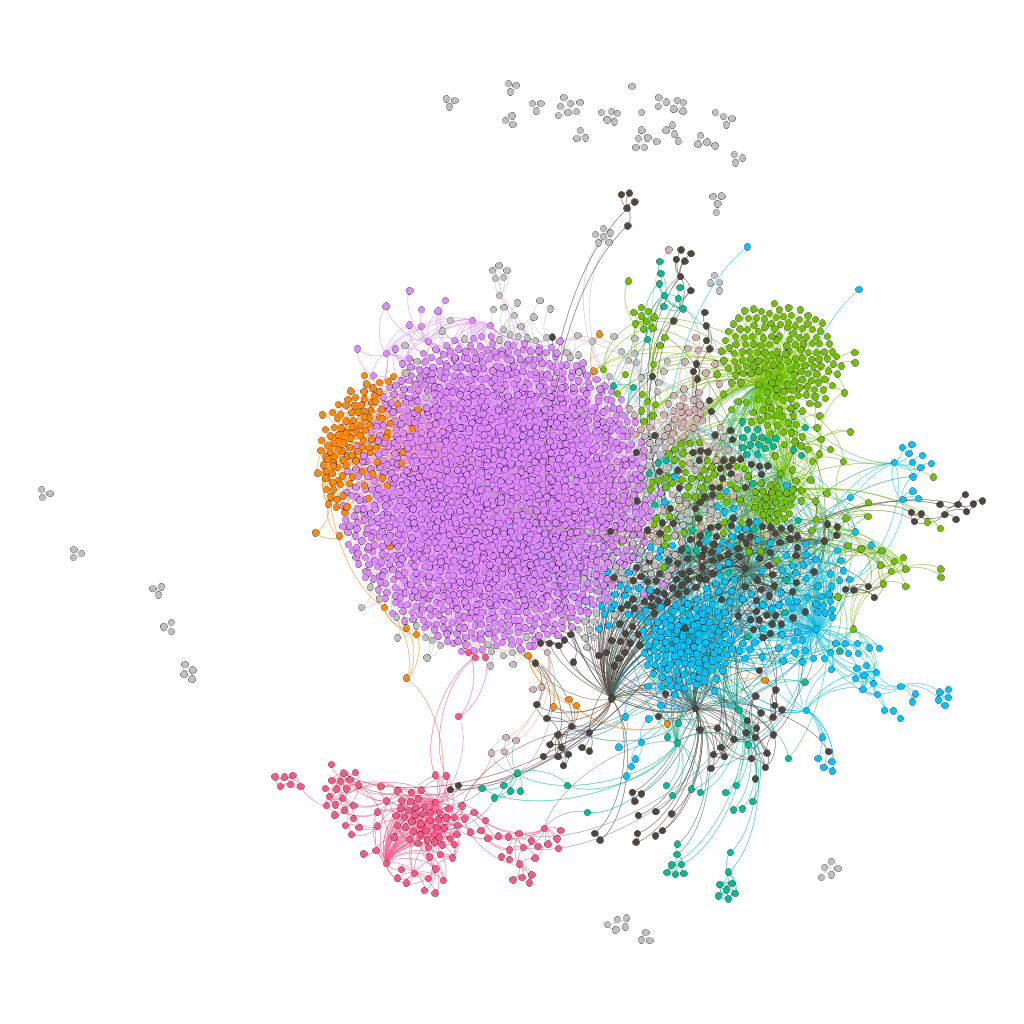
\includegraphics[width=\textwidth]{images/graph/communities.png}
    \caption{Comunidades identificadas en la red}
    \label{fig:communities}
\end{figure}

A primera vista, podemos identificar algunas de las comunidades descubiertas. La
de color morado es la correspondiente al \textit{tweet} con más interacciones,
siendo la verde y la azul las correspondientes a los otros dos con más
interacciones. Los nodos de color rojo son los de un conjunto de usuarios que
han puesto \textit{tweets} sobre el tema y han interaccionado solo entre ellos.
Además, la comunidad gris es la de islas completamente aisladas.

Las comunidades detectadas se corresponden de forma bastante fiel con las
agrupaciones de \textit{tweets} e interacciones que tenemos en la red, así que
consideramos que sí que tienen una influencia real en la red. La única comunidad
que no podemos identificar claramente es la de color negro.
